% ****** Start of file aipsamp.tex ******
%
%   This file is part of the AIP files in the AIP distribution for REVTeX 4.
%   Version 4.1 of REVTeX, October 2009
%
%   Copyright (c) 2009 American Institute of Physics.
%
%   See the AIP README file for restrictions and more information.
%
% TeX'ing this file requires that you have AMS-LaTeX 2.0 installed
% as well as the rest of the prerequisites for REVTeX 4.1
%
% It also requires running BibTeX. The commands are as follows:
%
%  1)  latex  aipsamp
%  2)  bibtex aipsamp
%  3)  latex  aipsamp
%  4)  latex  aipsamp
%
% Use this file as a source of example code for your aip document.
% Use the file aiptemplate.tex as a template for your document.
\documentclass[%
 aip,
 jmp,%
 amsmath,amssymb,
%preprint,%
 reprint,%
%author-year,%
%author-numerical,%
]{revtex4-1}

\usepackage{mathtools}
\usepackage{graphicx}% Include figure files
\usepackage{dcolumn}% Align table columns on decimal point
\usepackage{bm}% bold math
%\usepackage[mathlines]{lineno}% Enable numbering of text and display math
%\linenumbers\relax % Commence numbering lines
\usepackage{listings}
\usepackage{color} %red, green, blue, yellow, cyan, magenta, black, white
\definecolor{mygreen}{RGB}{28,172,0} % color values Red, Green, Blue
\definecolor{mylilas}{RGB}{170,55,241}
\linespread{1.25}
\renewcommand{\baselinestretch}{1.25}
\usepackage{float}
%\usepackage{dblfloatfix} 





\begin{document}


\preprint{AIP/123-QED}


\title[PHY319]{Dynamic Timescale Modelling of Globular Clusters}% Force line breaks with \\


\author{Jack Mayo}
 

\date{\today}% It is always \today, today,
             %  but any date may be explicitly specified

\begin{abstract}
Abstract \end{abstract}


\maketitle


\section{\label{sec:level1}Introduction}
Globular clusters (GCs) are groups of thousands of stars orbiting the Galactic centre with the individual stars gravitationally bound with a density higher than that of the galactic plane, located within 20 Kpc. In the Milky way alone there are 150 known GCs \cite{Harris1996}.Due to there abundance and distribution fitting a model to them would allow GC's to be used as standard candles for distances and ageing galaxies. GC formation is not well known so initial Mass and Radii are going to be varied for the model and will start modelling from a time at which the cluster as formed an equilibrium.  

GCs are useful tracers because they are abundant and bright making them easily observable in other galaxies. Stars within GCs were formed at the same time out of the same material making them the same population and metallicity and therefore ideal for Hertzsprung-Russel (HR) fitting for ageing the cluster. In order to use GCs as a tracer the physical parameters of the GC need to be modelled and fit to observed data. As we only see the cluster at a single point in time with no real changes during our observational timescale. Others at different stages in evolution can be observed and from this, knowledge of stellar evolution and dynamics we can build a model so that clusters can be used as a standard candle in ageing and distancing galaxies with resolvable globular clusters.%\cite{Heggie2007} 

globular cluster luminosity function
young clusters seem to be power law but dead now, old ones follow a gaussian not taking in to account galactic radius gives an unusual cut off. [CITATION NEEDED]
interpeting information by knowing how they die 

\begin{figure}[H]
\centering
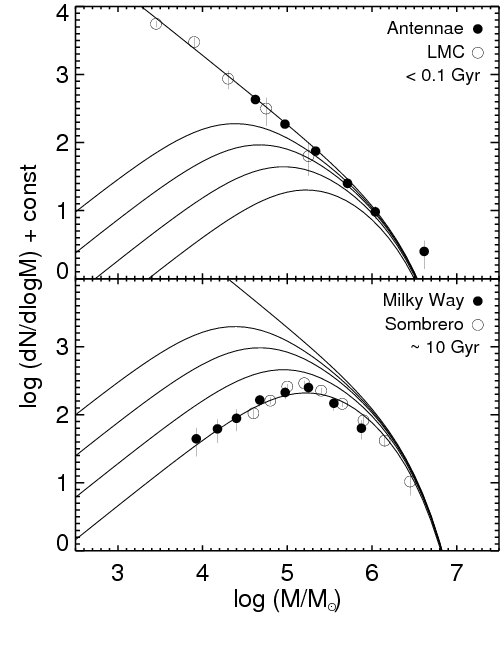
\includegraphics[width=0.45\textwidth]{GCmassfunction.png}
\caption{Mass distribution of GCs in young galaxiy (top) and older galaxy (bottom) The lines represent the model from Fall et al.\cite{Fall2009} which is not accurate however the points are correct. }
\label{massfunction}
\end{figure}

Figure \cite{massfunction} 

The evolution can be modelled in number of ways depending on what properties are to be determined.  The most explicit type of model is an N-body simulation where the stars are modelled as physical objects in a simulated space that evolve with time according to Newtonian dynamics and stellar evolution modelling of the individual stars, this takes a vast amount of computational power and time compared to other methods. Static models such as the Plummer and Jeans models solve a series of equations to find variable relationships. However Dynamical analytical models of specific clusters require significantly less computational power (Apart from N-body) and less parametrisation. The model in this paper is a Dynamical approach in which an initial mass function is assumed and the mass of the GC is calculated iteratively with respect to the mass loss mechanisms and initial parameters. As the N-body simulation is the most explicit comparing our model to the Baumgardt et al. 2003 simulations will give an idea of the accuracy of this method.





\section{\label{sec:level1}Method}

\subsection{\label{sec:level2}Mass Loss Mechanisms}
There are two main mass loss mechanisms for globular clusters, stellar evolution and dynamic mass loss. In stellar evolution, mass is lost due to internal dynamics of the star undergoing nuclear fusion creating ejecta as well as a small amount of mass lost as photons. As larger stars come to the end of their life and evolve into red giants ejecting their outer layers we discount that mass from the cluster dynamics for the over all cluster this gives the mass loss relationship over time as shown in equation \eqref{stellarevol}. The stellar evolution mass loss initially is large for a GC as the largest stars undergo fission at a greater rate.
This is dependent on metallicity `$Z$'modelled with $Z=0.0200$ \cite{Grevesse2010} which gives a set of constants from table \ref{table:constants} for eqn \eqref{stellarevol} \cite{Lamers2005}. 


\begin{equation}
\begin{aligned}
  &\log(q_{ev})=(\log(t)-a_{ev})^{b_{ev}} + c_{ev} \\
  & $t$>12.5 Myr. \label{stellarevol}
  \end{aligned}
\end{equation}

\begin{table}[h]
\caption{Table of constants used for Stellar evolution rates based on the metallicity of the Cluster \cite{Lamers2005}} % title of Table
\centering  % used for centering table
\begin{tabular}{c c c c} % centered columns (4 columns)
\hline\hline                        %inserts double horizontal lines
Z & $a_{ev}$ & $b_{ev}$ & $c_{ev}$  \\ [0.5ex] % inserts table 
%heading
\hline                  % inserts single horizontal line 
0.0004 & 7.06 & 0.265 & -1.790 \\
0.0040 & 7.06 & 0.260 & -1.800 \\
0,0080 & 7.03 & 0.260 & -1.800\\
0.0200 & 7.00 & 0.255 & -1.805 \\
0.0500 & 7.00 & 0.250 & -1.820 \\ [1ex]  % inserting body of the table
% [1ex] adds vertical space
\hline %inserts single line
\end{tabular}
\label{table:constants} % is used to refer this table in the text
\end{table}

Mass loss from the physical motion of the stars interacting gravitationally with each other causes an evaporation-like effect where stars gain enough energy from gravitational interactions to achieve an escape velocity [see appendix for derivation] The relaxation time ($t_{rlx}$) is the time in which the cluster loses $1\%$ of its mass through dynamics this is based on the crossing time ($t_{cross}$) the time it would take for a star with an average velocity to traverse the cluster. In this model all the stars that leave the cluster will do so with zero energy assuming a normal distribution of the energy of ejected stars with a zero mean this is not entirely accurate. This variable is dependent on the Radius and mass of the GC as the initial mass function and radius is not well understood these will be initial parameters of the simulation exploring how changes in mass and radius effect the lifetime of the GC. 

There are other mass loss mechanisms that effect GCs such as the position in the host galaxy which allows individual stars to be ejected at lower than the escape velocity due to external gravitational effects due to the host galaxy also the motion through the galactic plane causes a violent disruption effect of gravitational shock waves though the cluster. These are omitted from this simulation for a more general model.

\begin{equation}
  t_{rlx}= \frac{N}{8 \ln N}* t_{cross} \label{trelax}
\end{equation}

The mass loss can then be calculated from the initial parameters. Assuming energy is constant the virial theorem applies every step of the simulation the Energy remains the same so we can express the new quantities in terms of the previous.

\begin{equation}
  E=\frac{GM_{0}^{2}}{2R_{0}}=\frac{GM_{new}^{2}}{2R_{new}}
\label{energymass}
\end{equation}

Where `$M_{0}$' is original mass and `$M_{new}$' is the Mass after a time `$t$' and `$R_{0}$' is original mass and `$R_{new}$' is radius after time `$t$' and `$G$' is Newtons Gravitational constant. It is important to note that there is not a definite radius of a GC and there are two different ways that it can be expressed the \textbf{Tidal Radius} and the \textbf{Half Mass Radius} we are using the Half Mass Radius the radius in which half the mass is contained as opposed to the tidal radius of the cluster which is the radius at which the clusters gravity will be overcome by external gravitational forces. From theses the change in Mass affects number of stars in the cluster `$N$' and the relaxation time `$t_{rlx}$' and the change in `$R$' affects the crossing time `$t_{cross}$'. As we are defining `$M_{new}$' as `$ \delta M_{0}$' where `$\delta$' is `$1-mass step$` in this simulation `$0.99$'. This gives the new radius to be.

\begin{equation}
  \frac{1}{R_{0}}=\frac{\delta^{2}}{R_{new}}
\label{radius1}
\end{equation}

\begin{equation}
R_{new}=\delta^{2}R_{0}
\label{radius2}
\end{equation}

This can be fed into the virial theorem to produce initial relationship.

\begin{equation}
\frac{1}{2} M_{0} v_{0}^{2}=\frac{GM_{0}^{2}}{2R_{0}}
\label{crossing1}
\end{equation}
 
 Then newly derived quantities can be substituted in to find the relationship between `$v_{0}$' and `$v_{new}$'.
  
\begin{equation}
 \delta M_{0} v_{new}^{2}=\frac{G \delta^{2} M_{0}^{2}}{R_{0}}*\delta^{2}
\label{crossing2}
\end{equation}

Rearranging and substituting into eqn \eqref{crossing1}.

\begin{equation}
 \delta^{3} v_{old}^{2}=v_{new}^{2}
\label{crossing3}
\end{equation}

\begin{equation}
 \delta^{\frac{3}{2}} v_{old}=v_{new}
\label{crossing3}
\end{equation}

The crossing time is defined as.

\begin{equation}
 t_{cross0}=\frac{R_{0}}{v_{0}}
\label{crossing4}
\end{equation}

Then is substituted into eqn \eqref{crossing3}.

\begin{equation}
 t_{crossnew}=\frac{\delta^{2}R_{0}}{\delta^{-\frac{1}{2}}v_{0}}
\label{crossing5}
\end{equation}

Substituting this into eqn \eqref{trelax} 


\begin{equation}
  t_{rlxnew}= \frac{\ln N}{ \ln \delta N}* \delta^{\frac{7}{2}} t_{rlx0} \label{trelaxnew}
\end{equation}







\subsection{\label{sec:level2}The Dynamical Timescale}

\begin{figure*}[H]
\centering
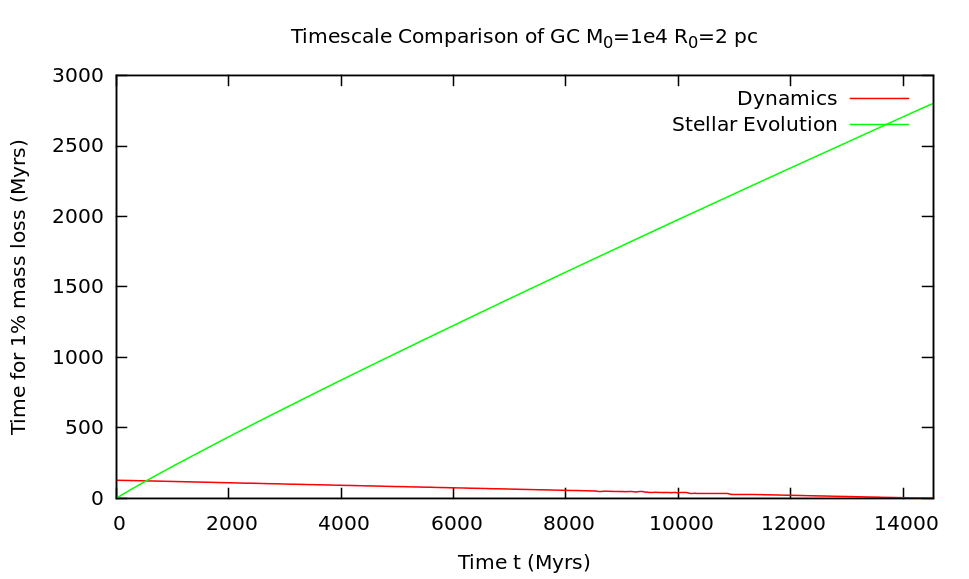
\includegraphics[width=1\textwidth]{fig4.png}
\caption{Time scales. \cite{Lamers2005}}
\label{timescale}
\end{figure*}

The dynamical timescale in stellar physics is defined as the shortest amount of time in which a system can undergo change. The  dynamical timescale in a GC was defined as the time in which the GC can lose one percent of its mass, however this varies throughout the lifetime of the cluster as the different mass loss mechanisms change effectiveness. This timescale allows the system to simulate the cluster getting into equilibrium state between each mass calculation and reduces the time for the simulation whilst ensuring that important features, such as rapid changes in mass, are graphed with an high resolution. 






\subsection{\label{sec:level2}Simulation Method}
As the timescales are properties of initial conditions, the time taken to lose $1\%$ of the cluster mass is calculated separately for both mechanisms, they are then compared to see which one is the significant timescale `$t_{small}$' ie the smaller time, then the mass loss from the less significant time scale `$t_{large}$' is calculated assuming a linear mass loss over the small time. The total Mass loss is then calculated using \eqref{totalmassloss}.


\begin{equation}
  \Delta M_{total}=0.01 M_{0}+\frac{t_{large}}{t_{small}}*0.01 M_{0}
  \label{totalmassloss}
\end{equation}

The time is then increased by the significant timescale with the new mass and radius then the timescales calculated again. This way the mass loss for each point is between $1\%$ and $2\%$ the original mass of the cluster. The code can be seen in the appendix 



\section{\label{sec:level1}Analysis}

\begin{figure*}[t]
\centering
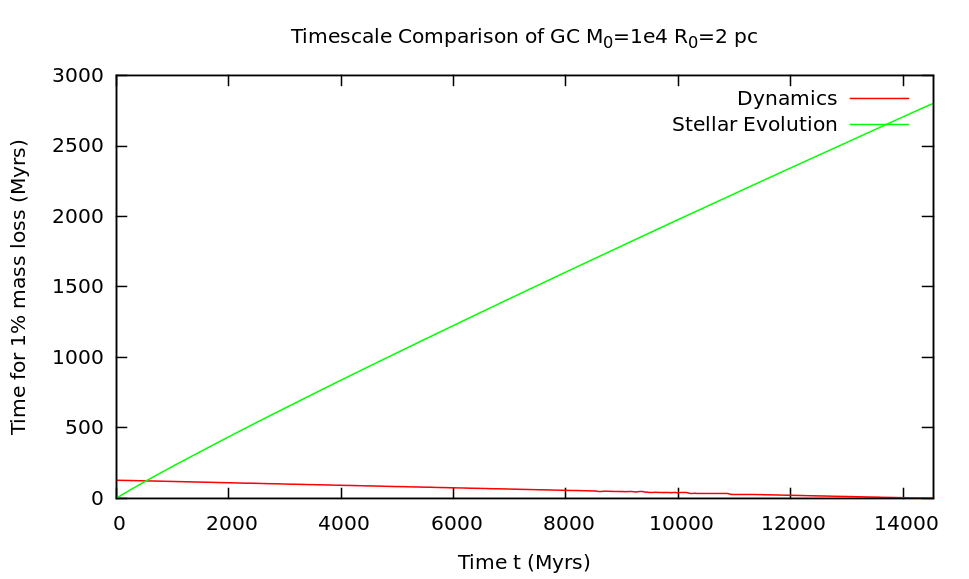
\includegraphics[width=1\textwidth]{fig4.png}
\caption{Time scales. \cite{Lamers2005}}
\label{timescale}
\end{figure*}

Do a metallicity comparison here 







\begin{figure*}[t]
\centering
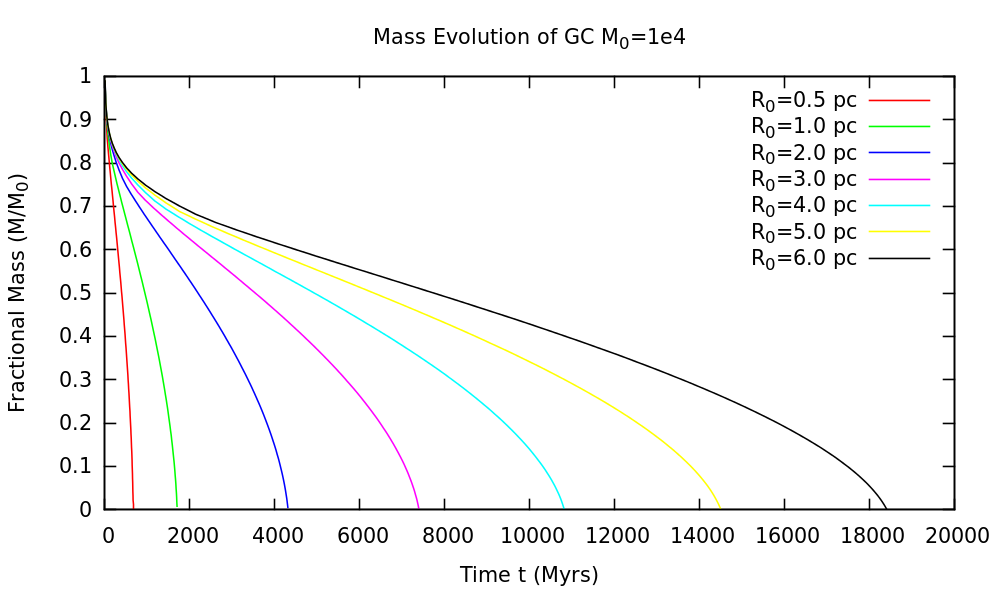
\includegraphics[width=1\textwidth]{fig2.png}
\caption{Evolution of a GC of various Radii.}
\label{constmassvarradii}
\end{figure*}

\begin{figure*}[t]
\centering
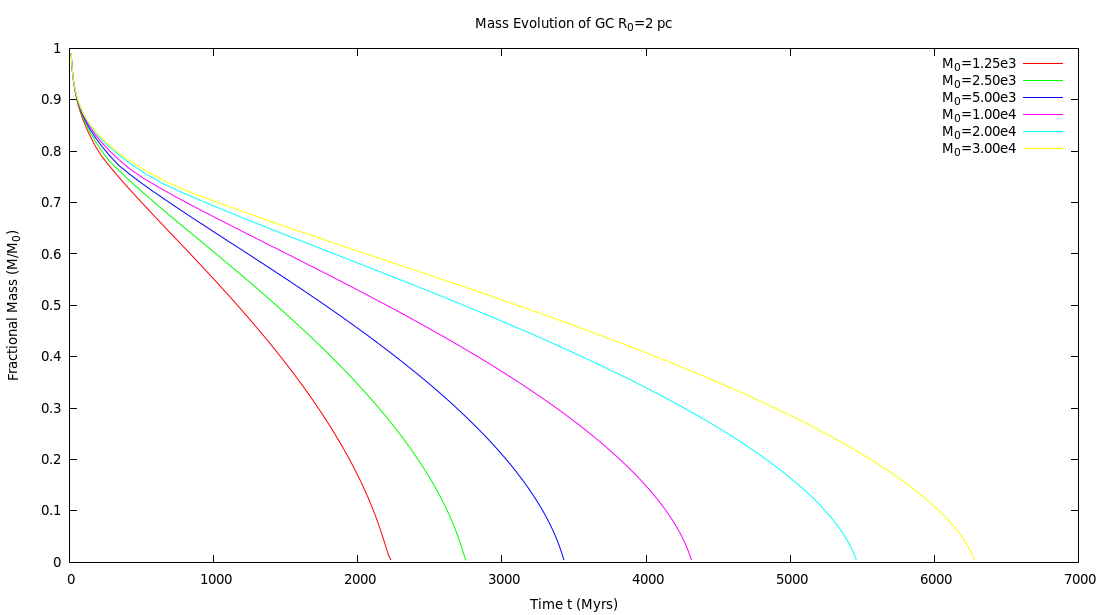
\includegraphics[width=1\textwidth]{fig1.png}
\caption{Evolution of a GC of various Masses.}
\label{varmassconstradii}
\end{figure*}


\section{\label{sec:level1}Conclusion}
The models presented are not fitted to any actual clusters given more time the model could be expanded to include the other mass loss mechanisms and fit to observational data. The model could also be expanded to include the common observational quantities such as surface luminosity and absolute magnitudes. There is some argument over the metallicity of stars in GCs, in this model it is assumed to be approximately the solar metallicity. However observational quantities disagree with this as shown in section \ref{observed} this is not entirely accurate but is easily rectified by using the correct set of constants for eqn \eqref{stellarevol} founf in table \ref{table:constants}.
Further modelling - fitting observational data discuss differences in observational quantities to what we have modelled. also inclusion of Galactic forces and energy loss
[METALLICITY]

\clearpage
\bibliographystyle{plain}
\bibliography{library.bib}
\section{Appendix}\label{appendix}
\subsubsection{Compiler details}\label{compiler}

MinGw gcc using the Eclipse Luna IDE and inbuilt CDT Toolchain. All code is hosted on DCVS https://github.com/jackomayo/clusterdynamics.git


\subsubsection{Main Program}\label{code}
Newtons gravitational constant has been calculated in terms of $PC^{3}M_{\sun}^{-1}yr^{-2}$ for sanity's sake.

%\lstinputlisting[language=c++]{main.cpp}

\subsubsection{Observational features of Globular Clusters}\label{observed}
Info on metallicity and sizes of GC's and shiit

do it with 2 different metallicity plots 

\end{document}
%
% ****** End of file aipsamp.tex ******
\